\chapter{المدارات الجزيئية للجزيئات الثنائية الذرة}\label{ch:b2:diatomic-mos}

اسكب الأكسجين السائل بين قطبي مغناطيس قوي فينجذب
جانبًا؛ أما النيتروجين السائل فيسقط مستقيمًا. فجزيء الأكسجين يحمل
إلكترونات منفردة يجذبها المجال المغناطيسي. وبنية لويس له،
\ce{O=O} وكل إلكتروناتها مقترنة، لا تستطيع أن تقول ذلك. أما \omterm{def:b2:diatomic-mos:lcao}{المدارات الجزيئية}،
المبنية من المدارات الذرية في الفصل السابق، فتضع كل إلكترون
في الجزيء في مستوى خاص به: فهي تفسر مغناطيسية
الأكسجين، وقوة الروابط وأطوالها، والطاقات اللازمة
لتأيين الجزيئات --- وتمهد لدراسة التفاعلية في
الفصول التالية.

\begin{recall}
\Cref{ch:b2:atomic-orbitals}: المدارات الذرية، وأشكالها وإشاراتها
وطاقاتها. ومجلد السنة الأولى: بنى لويس، والرابطتان $\sigma$ و$\pi$ بوصفهما
مفهومين وصفيين، والتهجين وحدوده، والإلكترونات المنفردة
والجذور الحرة.
\end{recall}

\begin{omfigure}
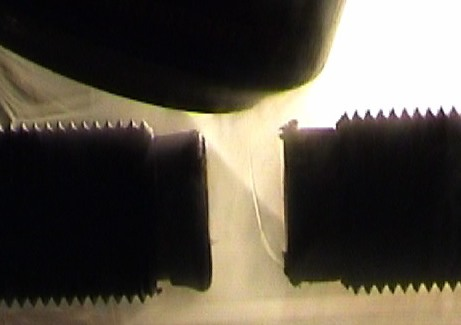
\includegraphics[width=0.42\linewidth]{images/book3/liquid-oxygen.jpg}

{\small خيط رفيع من الأكسجين السائل، يسقط بين قطبي مغناطيس
قوي، فينجذب نحوهما ويبقى معلقًا كالجسر: فالجزيء
\omterm{def:b2:diatomic-mos:magnetism}{بارامغناطيسي}. (صورة: بيتر كاوبر، ملكية عامة، ويكيميديا كومنز.)}
\end{omfigure}

\section{طريقة LCAO}

\begin{definition}[المدار الجزيئي]\label{def:b2:diatomic-mos:lcao}
\emph{المدار الجزيئي}\index{مدار جزيئي} هو \omterm{def:b2:atomic-orbitals:wavefunction}{الدالة الموجية} لإلكترون واحد
في جزيء، ممتدة على كل أنويته. وفي طريقة \emph{LCAO}\index{LCAO}
(التركيب الخطي للمدارات الذرية) يُكتب مجموعًا لمدارات ذرية
لذرات الجزيء، $\psi = \sum_i c_i\varphi_i$، بمعاملات مختارة
تجعل الطاقة أدنى ما يمكن.
\end{definition}

من أجل ذرتين A وB، تأتي كل منهما بمدار واحد، $\psi = c_A\varphi_A + c_B\varphi_B$.
وطاقة إلكترون في $\psi$، بعد جعلها صغرى بالنسبة إلى المعاملات،
تُدخل ثلاثة أعداد.

\begin{definition}[تكاملات طريقة LCAO]\label{def:b2:diatomic-mos:integrals}
من أجل مدارين ذريين حقيقيين $\varphi_A$ و$\varphi_B$ ومؤثر الطاقة $\hat H$
لإلكترون في الجزيء:
\begin{itemize}
  \item يقيس \emph{تكامل التداخل}\index{تكامل التداخل} $S = \int\varphi_A\varphi_B\,dV$
        مقدار اشتغال المدارين المنطقةَ نفسها ($S = 1$ لمدارين
        متطابقين منطبقين)؛
  \item \emph{تكامل كولوم}\index{تكامل كولوم} $\alpha_A = \int\varphi_A\hat
        H\varphi_A\,dV$ هو طاقة إلكترون في $\varphi_A$ داخل الجزيء،
        وهي قريبة من طاقة المدار الذري؛
  \item \emph{تكامل الرنين}\index{تكامل الرنين} $\beta = \int\varphi_A\hat
        H\varphi_B\,dV$، وهو سالب، يقيس اقتران المدارين.
\end{itemize}
طاقات \omterm{def:b2:diatomic-mos:lcao}{المدارات الجزيئية} $E$ هي جذور \emph{المحدد
القرني}\index{محدد قرني}
\[
  \begin{vmatrix} \alpha_A - E & \beta - ES \\ \beta - ES & \alpha_B - E \end{vmatrix} = 0 .
\]
\end{definition}

يأتي المحدد من جعل $E = \int\psi\hat H\psi\,dV/\int\psi^2\,dV$ صغرى
بالنسبة إلى $c_A$ و$c_B$: فالشرطان $\partial E/\partial c_A =
\partial E/\partial c_B = 0$ يكوّنان جملة خطية متجانسة، ليس لها حل غير معدوم
إلا إذا انعدم محددها. ونقبل هذه الخطوة التغيرية
هنا.

\begin{theorem}[مداران متماثلان]\label{thm:b2:diatomic-mos:homonuclear}
من أجل $\alpha_A = \alpha_B = \alpha$، يكون \omterm{def:b2:diatomic-mos:lcao}{المداران الجزيئيان}
\[
  E_+ = \frac{\alpha + \beta}{1 + S}, \quad \psi_+ = \frac{\varphi_A + \varphi_B}{\sqrt{2(1 + S)}} ;
  \qquad
  E_- = \frac{\alpha - \beta}{1 - S}, \quad \psi_- = \frac{\varphi_A - \varphi_B}{\sqrt{2(1 - S)}} .
\]
\end{theorem}

\begin{proof}
يعطي المحدد $(\alpha - E)^2 = (\beta - ES)^2$، ومنه $\alpha - E = \pm(\beta - ES)$.
مع إشارة الجمع، $E(1 + S) = \alpha + \beta$؛ ومع إشارة الطرح، $E(1 - S) = \alpha
- \beta$. وبالعودة إلى الجملة الخطية، تعطي $(\alpha - E)c_A + (\beta - ES)c_B = 0$ $c_B
= c_A$ من أجل $E_+$ و$c_B = -c_A$ من أجل $E_-$. والتنظيم: $\int(\varphi_A \pm
\varphi_B)^2\,dV = 2 \pm 2S$.
\end{proof}

\begin{definition}[المدارات الرابطة والمضادة للربط]\label{def:b2:diatomic-mos:bonding}
\emph{المدار الرابط}\index{مدار رابط} يقع تحت المدارات الذرية التي
يتكوّن منها: فتتراكم كثافته الإلكترونية بين النواتين. و\emph{المدار
المضاد للربط}\index{مدار مضاد للربط} يقع فوقها وله
مستوٍ عقدي بين النواتين. و\emph{المدار غير الرابط}\index{مدار غير رابط}
يحتفظ بطاقة المدار الذري، الذي لا يجد شريكًا
يتركب معه.
\end{definition}

\begin{proposition}[المدار المضاد للربط يرتفع أكثر]\label{prop:b2:diatomic-mos:asymmetry}
من أجل $S > 0$، يرتفع المستوى المضاد للربط فوق $\alpha$ بأكثر مما
ينخفض المستوى الرابط تحته.
\end{proposition}

\begin{proof}
$E_+ - \alpha = (\beta - \alpha S)/(1 + S)$ و$E_- - \alpha = -(\beta - \alpha S)/(1 - S)$.
والبسط $\beta - \alpha S$ سالب (فالاقتران هو الغالب)، و$1 - S < 1
+ S$: فالإزاحة الثانية أكبر بالقيمة المطلقة.
\end{proof}

مع إلكترونين، كما في \ce{H2}، يدخل كلاهما $\psi_+$ فيكون الجزيء أكثر
استقرارًا من الذرتين المنفصلتين. ومع أربعة، كما في \ce{He2}، يجب أن يدخل اثنان $\psi_-$،
وهو ما يكلّف أكثر مما يكسبه $\psi_+$: فالجزيء \ce{He2} غير مرتبط.

\begin{omfigure}
\begin{MOdiagram}[names, labels]
  \atom[H]{left}{ 1s = {0;up} }
  \atom[H]{right}{ 1s = {0;up} }
  \molecule[\ce{H2}]{ 1sMO = {.75;pair} }
\end{MOdiagram}
\hspace{1.5cm}
\begin{MOdiagram}[names, labels]
  \atom[He]{left}{ 1s = {0;pair} }
  \atom[He]{right}{ 1s = {0;pair} }
  \molecule[\ce{He2}]{ 1sMO = {.75;pair,pair} }
\end{MOdiagram}

{\small مخططا \omterm{def:b2:diatomic-mos:lcao}{المدارات الجزيئية} للجزيئين \ce{H2} (\omterm{def:b2:diatomic-mos:bond-order}{رتبة الرابطة} 1) و\ce{He2} (\omterm{def:b2:diatomic-mos:bond-order}{رتبة
الرابطة} 0، غير مرتبط). كل صندوق مستوى يحمل إلكترونين على الأكثر
متعاكسي السبين؛ وتصل الخطوط المتقطعة كل \omterm{def:b2:diatomic-mos:lcao}{مدار جزيئي} بالمدارات الذرية
التي بُني منها.}
\end{omfigure}

\section{التداخل والتناظر}

\begin{definition}[المداران $\sigma$ و$\pi$]\label{def:b2:diatomic-mos:sigma-pi}
\emph{مدار $\sigma$}\index{مدار سيغما@مدار $\sigma$} لجزيء خطي لا يتغير بأي
دوران حول المحور الجزيئي: فليس له مستوٍ عقدي يحوي المحور.
و\emph{مدار $\pi$}\index{مدار باي@مدار $\pi$} يغيّر إشارته بدوران قدره $180^\circ$ حول
المحور: فله مستوٍ عقدي واحد يحوي المحور. وتميّز نجمةٌ المداراتِ
المضادة للربط ($\sigma^*$، $\pi^*$).
\end{definition}

\begin{proposition}[تداخل معدوم بسبب التناظر]\label{prop:b2:diatomic-mos:symmetry}
المداران اللذان يكون أحدهما متناظرًا والآخر ضد متناظر بالنسبة إلى
مستوٍ يحوي المحور الجزيئي تداخلهما معدوم وتكامل رنينهما
معدوم: فلا يتركبان.
\end{proposition}

\begin{proof}
الانعكاس في المستوي يترك الفضاء دون تغيير لكنه يحوّل الجداء
$\varphi_A\varphi_B$ إلى معاكسه عند النقطة المرآوية: فتُختصر مساهمتا
نصفي الفضاء في $\int\varphi_A\varphi_B\,dV$. ويصح الأمر نفسه على
$\int\varphi_A\hat H\varphi_B\,dV$، لأن للمؤثر $\hat H$ تناظر الجزيء.
\end{proof}

يتآثر مداران بقوة حين يكون لهما التناظر نفسه (تداخل غير
معدوم)، ويتداخلان جيدًا، ويقعان عند طاقتين متقاربتين. فالمدار 1s لإحدى الذرتين 
و$2\mathrm p_x$ للأخرى ($x$ عمودي على المحور) لا يتركبان أبدًا؛
والمداران $2\mathrm p_z$ (على طول المحور) يعطيان مدارات $\sigma$؛ و$2\mathrm p_x$ 
و$2\mathrm p_y$ يعطيان زوجين من مدارات $\pi$ متساوية الطاقة.

\begin{omfigure}
\begin{tikzpicture}[font=\small]
  % sigma 1s
  \pic at (0,0) {oms={0.85}}; \pic at (0.7,0) {oms={0.85}};
  \node at (0.35,-0.75) {$\sigma_{1s}$};
  \pic at (2.2,0) {oms={0.85}}; \pic at (2.9,0) {oms={-0.85}};
  \node at (2.55,-0.75) {$\sigma^*_{1s}$};
  % sigma 2p
  \pic at (4.6,0) {omp={-1}{0}}; \pic at (5.6,0) {omp={1}{0}};
  \node at (5.1,-0.75) {$\sigma_{2p}$};
  \pic at (7.4,0) {omp={-1}{0}}; \pic at (8.6,0) {omp={-1}{0}};
  \node at (8.0,-0.75) {$\sigma^*_{2p}$};
  % pi 2p
  \pic at (10.2,0) {omp={1}{90}}; \pic at (10.9,0) {omp={1}{90}};
  \node at (10.55,-0.95) {$\pi_{2p}$};
  \pic at (12.2,0) {omp={1}{90}}; \pic at (12.9,0) {omp={-1}{90}};
  \node at (12.55,-0.95) {$\pi^*_{2p}$};
  \draw[black!40, dashed] (-0.6,0) -- (13.4,0);
\end{tikzpicture}

{\small \omterm{def:b2:diatomic-mos:lcao}{المدارات الجزيئية} لجزيء ثنائي الذرة متجانس النوى، رسم تخطيطي (المحور
الجزيئي أفقي ومتقطع). التراكيب المتوافقة الطور (الرابطة) تجمع
اللون نفسه بين النواتين؛ والتراكيب المتعاكسة الطور (المضادة للربط) تضع
مستويًا عقديًا بينهما. ومدارات $\sigma$ متناظرة حول المحور؛ ولكل مدار $\pi$
المحور في مستويه العقدي.}
\end{omfigure}

\section{الجزيئات الثنائية الذرة المتجانسة النوى في الدورة 2}

بالمدارين 2s و2p لذرتين من الدورة 2 تتكوّن ثمانية \omterm{def:b2:diatomic-mos:lcao}{مدارات جزيئية}:
$\sigma_{2s}$، $\sigma^*_{2s}$، $\sigma_{2p}$، ومداران $\pi_{2p}$، ومداران $\pi^*_{2p}$،
و$\sigma^*_{2p}$.

\begin{proposition}[مزج s--p]\label{prop:b2:diatomic-mos:sp-mixing}
من أجل \ce{O2} و\ce{F2} يكون الترتيب \babelsublr{$\sigma_{2s} < \sigma^*_{2s} < \sigma_{2p} < \pi_{2p} <
\pi^*_{2p} < \sigma^*_{2p}$}. ومن أجل \ce{Li2} حتى \ce{N2}، التي يتقارب فيها المستويان 2s و2p،
تمتزج مدارات $\sigma$ المبنية من 2s و$2\mathrm p_z$: فيُدفع $\sigma_{2p}$ إلى أعلى فوق
$\pi_{2p}$.
\end{proposition}

\begin{proof}[تعليل]
للمدارين $\sigma_{2s}$ و$\sigma_{2p}$ التناظر نفسه فيمكن أن يتركب أحدهما مع
الآخر. والمستويان المتماثلا التناظر يتنافران (\cref{thm:b2:diatomic-mos:heteronuclear}
أدناه): فينخفض $\sigma_{2s}$، ويرتفع $\sigma_{2p}$، ويشتد ذلك كلما تقاربا. والفجوة
2s--2p تكبر على طول الدورة، فيكون الأثر كبيرًا في اليسار وصغيرًا في
الأكسجين والفلور. والتقاطع بين النيتروجين والأكسجين نقبله من
أطياف الإلكترونات الضوئية المقيسة.
\end{proof}

\begin{definition}[رتبة الرابطة]\label{def:b2:diatomic-mos:bond-order}
\emph{رتبة الرابطة}\index{رتبة الرابطة} لجزيء ثنائي الذرة هي $b = (n_b -
n_a)/2$، حيث $n_b$ و$n_a$ عددا الإلكترونات في \omterm{def:b2:diatomic-mos:bonding}{المدارات الرابطة} \omterm{def:b2:diatomic-mos:bonding}{والمدارات
المضادة للربط}.
\end{definition}

\begin{proposition}[رتبة الرابطة والرابطة]\label{prop:b2:diatomic-mos:bond-order}
بين ذرات الزوج نفسه من العناصر، تقترن \omterm{def:b2:diatomic-mos:bond-order}{رتبة الرابطة} الأعلى برابطة
أقصر وأقوى؛ \omterm{def:b2:diatomic-mos:bond-order}{ورتبة الرابطة} المعدومة تعني انعدام الرابطة.
\end{proposition}

\begin{proof}[تعليل]
كل إلكترون رابط يضيف كثافة بين النواتين ويخفض الطاقة؛
وكل إلكترون مضاد للربط يزيلها ويرفع الطاقة بقدر لا يقل عن ذلك
(\cref{prop:b2:diatomic-mos:asymmetry}). فالعدد الصافي للأزواج الرابطة يقيس
الارتباط. ولا تكون المقارنة ذات معنى إلا لذرات متشابهة: \omterm{def:b2:diatomic-mos:bond-order}{فرتبة الرابطة} في \ce{Li2}
1 مثل \ce{F2}، لكن مداراته 2s أكبر بكثير.
\end{proof}

\begin{definition}[البارامغناطيسية والدايامغناطيسية]\label{def:b2:diatomic-mos:magnetism}
تكون المادة \emph{بارامغناطيسية}\index{بارامغناطيسي} إذا كانت في جزيئاتها
إلكترونات منفردة: فتنجذب إلى داخل المجال المغناطيسي. وتكون
\emph{دايامغناطيسية}\index{دايامغناطيسي} إذا كانت كل إلكتروناتها مقترنة: فتُدفع
إلى خارج المجال دفعًا ضعيفًا.
\end{definition}

\begin{omfigure}
\begin{MOdiagram}[names, labels, style=square, distance=4.2cm, labels-fs=\scriptsize]
  \atom[N]{left}{ 2s = {0;pair}, 2p = {3.5;up,up,up} }
  \atom[N]{right}{ 2s = {0;pair}, 2p = {3.5;up,up,up} }
  \molecule[\ce{N2}]{ 2sMO = {.7;pair,pair}, 2pMO = {0.4/2.5,1.4;pair,pair,pair} }
\end{MOdiagram}
\hfill
\begin{MOdiagram}[names, labels, style=square, distance=4.2cm, labels-fs=\scriptsize]
  \atom[O]{left}{ 2s = {0;pair}, 2p = {3.5;pair,up,up} }
  \atom[O]{right}{ 2s = {0;pair}, 2p = {3.5;pair,up,up} }
  \molecule[\ce{O2}]{ 2sMO = {.7;pair,pair}, 2pMO = {1.8,.8;pair,pair,pair,up,up} }
\end{MOdiagram}

{\small مخططا \omterm{def:b2:diatomic-mos:lcao}{المدارات الجزيئية} التكافؤية للجزيئين \ce{N2} (يمينًا، مع مزج s--p:
$\sigma_{2p}$ فوق $\pi_{2p}$) و\ce{O2} (يسارًا). النيتروجين: \omterm{def:b2:diatomic-mos:bond-order}{رتبة الرابطة}
$(8 - 2)/2 = 3$، وكل الإلكترونات مقترنة. الأكسجين: \omterm{def:b2:diatomic-mos:bond-order}{رتبة الرابطة} $(8 - 4)/2 = 2$، مع إلكترونين
منفردين في المدارين $\pi^*$ (قاعدة هوند): فالجزيء \ce{O2}
\omterm{def:b2:diatomic-mos:magnetism}{بارامغناطيسي}. ويأخذ المخططان $x$ محورًا جزيئيًا، ومن هنا الرموز
$2\sigma_x$، $2\pi_y$، $2\pi_z$.}
\end{omfigure}

\begin{method}[بناء مخطط مدارات جزيئية وملؤه]\label{met:b2:diatomic-mos:build-diagram}
\begin{enumerate}
  \item ضع المدارات الذرية التكافؤية لكل ذرة عند طاقاتها، والذرة الأكثر
        كهرسلبية أدنى.
  \item ركّب المدارات المتماثلة التناظر: كل زوج يعطي \omterm{def:b2:diatomic-mos:bonding}{مدارًا رابطًا}
        تحتهما \omterm{def:b2:diatomic-mos:bonding}{ومدارًا مضادًا للربط} فوقهما؛ والمدار الذي بلا شريك يبقى
        غير رابط.
  \item في الجزيئات المتجانسة النوى من الدورة 2، استعمل الترتيب الذي يكون فيه $\sigma_{2p}$ فوق
        $\pi_{2p}$ حتى النيتروجين، وتحته ابتداءً من الأكسجين.
\end{enumerate}
\end{method}

\begin{method}[قراءة مخطط مملوء]\label{met:b2:diatomic-mos:fill}
\begin{enumerate}
  \item عدّ إلكترونات التكافؤ (أضف واحدًا لكل شحنة سالبة، واطرح واحدًا
        لكل شحنة موجبة).
  \item املأ من الأسفل، إلكترونين لكل مدار، مع قاعدة هوند للمستويات
        المتساوية الطاقة.
  \item \omterm{def:b2:diatomic-mos:bond-order}{رتبة الرابطة} $(n_b - n_a)/2$؛ والإلكترونات المنفردة تعطي \omterm{def:b2:diatomic-mos:magnetism}{البارامغناطيسية}.
  \item أعلى مستوى مشغول هو الذي يتأين أولًا.
\end{enumerate}
\end{method}

\begin{omfigure}
\small
\renewcommand{\arraystretch}{1.15}
\begin{tabular}{lcccccc}
 & \ce{Li2} & \ce{C2} & \ce{N2} & \ce{O2} & \ce{F2} & \ce{NO} \\ \hline
إلكترونات التكافؤ & 2 & 8 & 10 & 12 & 14 & 11 \\
\omterm{def:b2:diatomic-mos:bond-order}{رتبة الرابطة} & 1 & 2 & 3 & 2 & 1 & 2.5 \\
إلكترونات منفردة & 0 & 0 & 0 & 2 & 0 & 1 \\
طول الرابطة $r_e$ (pm) & 267.3 & 124.3 & 109.8 & 120.8 & 141.2 & 115.1 \\
\babelsublr{$D_0$ (\unit{eV})} & 1.04 & 6.15 & 9.76 & 5.12 & 1.60 & 6.51 \\
\end{tabular}

\smallskip
{\small الجزيئات الثنائية الذرة في الدورة 2: رتب الروابط من مخططات \omterm{def:b2:diatomic-mos:lcao}{المدارات الجزيئية}؛ وأطوال
الروابط من المطيافية، وطاقات التفكك $D_0$ من أنتالبيات التكوين المجدولة
عند \qty{0}{K}، $D_0 = \Delta_f H_0(\mathrm A) + \Delta_f H_0(\mathrm B) - \Delta_f
H_0(\mathrm{AB})$.}
% ledger: re:Li2, re:C2, re:N2, re:O2, re:F2, re:NO, janafH0:Li, janafH0:Li2, janafH0:C, janafH0:C2, janafH0:N, janafH0:O, janafH0:F, janafH0:NO
\end{omfigure}

\section{الجزيئات الثنائية الذرة غير المتجانسة النوى}

\begin{theorem}[مداران مختلفا الطاقة]\label{thm:b2:diatomic-mos:heteronuclear}
من أجل $\alpha_A > \alpha_B$ (B أكثر كهرسلبية)، مع إهمال $S$، و$\bar\alpha = (\alpha_A
+ \alpha_B)/2$ و$\Delta = \alpha_A - \alpha_B$:
\[
  E_\mp = \bar\alpha \mp \sqrt{\Delta^2/4 + \beta^2} .
\]
\omterm{def:b2:diatomic-mos:bonding}{للمدار الرابط} (الأدنى) معامله الأكبر على B، وللمدار المضاد للربط
على A؛ وحين $\Delta \gg |\beta|$، يكون $E_- \approx \alpha_B - \beta^2/\Delta$ و$E_+
\approx \alpha_A + \beta^2/\Delta$.
\end{theorem}

\begin{proof}
مع $S = 0$ تكون الطاقات القيم الذاتية للمصفوفة \babelsublr{$\begin{pmatrix}\alpha_A & \beta \\
\beta & \alpha_B\end{pmatrix}$}: $(\alpha_A - E)(\alpha_B - E) = \beta^2$، وجذراها
$\bar\alpha \pm \sqrt{\Delta^2/4 + \beta^2}$. ومن أجل الجذر الأدنى، $(\alpha_B - E_-)c_B = -\beta
c_A$؛ و$\alpha_B - E_- = \sqrt{\Delta^2/4 + \beta^2} - \Delta/2$ أصغر من $|\beta|$، ومنه
$|c_A| < |c_B|$. ومن أجل $\Delta \gg |\beta|$، $\sqrt{\Delta^2/4 + \beta^2} \approx \Delta/2 +
\beta^2/\Delta$.
\end{proof}

\begin{omfigure}
\begin{tikzpicture}
\begin{axis}[width=0.55\linewidth, height=6cm, xmin=0, xmax=8, ymin=-5, ymax=5,
  axis x line=bottom, axis y line=left, xlabel={$\Delta/|\beta|$}, ylabel={$E/|\beta|$},
  tick label style={font=\small}, label style={font=\small}]
\addplot[omThm, thick] table[x=d, y=Ehigh] {figdata/out/bachelor-2-two-level-a.dat};
\addplot[omDef, thick] table[x=d, y=Elow] {figdata/out/bachelor-2-two-level-a.dat};
\addplot[black!50, densely dotted] table[x=d, y=aA] {figdata/out/bachelor-2-two-level-a.dat};
\addplot[black!50, densely dotted] table[x=d, y=aB] {figdata/out/bachelor-2-two-level-a.dat};
\addplot[omThm, dashed] table[x=d, y=Phigh] {figdata/out/bachelor-2-two-level-a-pert.dat};
\addplot[omDef, dashed] table[x=d, y=Plow] {figdata/out/bachelor-2-two-level-a-pert.dat};
\node[font=\scriptsize, black!60, anchor=north west] at (axis cs:5.5,2.6) {$\alpha_A$};
\node[font=\scriptsize, black!60, anchor=south west] at (axis cs:5.5,-2.6) {$\alpha_B$};
\node[font=\scriptsize, omThm, anchor=south east] at (axis cs:3.2,2.2) {مضاد للربط};
\node[font=\scriptsize, omDef, anchor=north east] at (axis cs:3.2,-2.2) {رابط};
\end{axis}
\end{tikzpicture}

{\small مستويان متآثران. كلما كبرت الفجوة $\Delta$ بين المدارين الذريين،
اقتربت المستويات الجزيئية (المتصلة) من المستويات الذرية (المنقّطة): فيصير الاستقرار
$\beta^2/\Delta$ في حد الاضطراب (المتقطع) صغيرًا. وعند $\Delta = 0$ يكون
الانشطار $2|\beta|$.}
\end{omfigure}

في فلوريد الهيدروجين يلاقي المدار 1s للهيدروجين مدارات 2p للفلور الأدنى
بكثير. ولا يملك التناظر المناسب إلا $2\mathrm p_z$، على طول المحور: فيكوّن
\omterm{def:b2:diatomic-mos:bonding}{مدارًا رابطًا} $\sigma$ مرجَّحًا على الفلور، ومدارًا $\sigma^*$ مرجَّحًا على
الهيدروجين. ويبقى المداران $2\mathrm p_x$ و$2\mathrm p_y$ للفلور
غير رابطين: فهما زوجاه الحران. والرابطة مستقطبة نحو الفلور.

لأحادي أكسيد الكربون إلكترونات التكافؤ العشرة نفسها التي في \ce{N2} ومخطط مشابه،
لكن مدارات الأكسجين تقع أدنى. \omterm{def:b2:diatomic-mos:bonding}{فمداراته الرابطة} مرجَّحة على الأكسجين؛
وأعلى مداراته المشغولة، وهو مدار $\sigma$ مرجَّح على الكربون، زوج حر
على الكربون. ولذلك يرتبط أحادي أكسيد الكربون بالفلزات عبر الكربون
(\cref{ch:b2:coordination-complexes}).

\begin{omfigure}
\begin{tikzpicture}[font=\small]
  % CO schematic: C left (higher), O right (lower)
  \pic (c2s) at (0,0.6) {omlevel={ud}{0.8}}; \node[left] at (-0.5,0.6) {2s};
  \pic (c2p1) at (-0.45,2.6) {omlevel={u}{0.4}}; \pic (c2p2) at (0,2.6) {omlevel={u}{0.4}}; \pic (c2p3) at (0.45,2.6) {omlevel={empty}{0.4}};
  \node[left] at (-0.75,2.6) {2p};
  \node at (0,-0.6) {C};
  \pic (o2s) at (6,-1.2) {omlevel={ud}{0.8}}; \node[right] at (6.5,-1.2) {2s};
  \pic (o2p1) at (5.55,1.4) {omlevel={ud}{0.4}}; \pic (o2p2) at (6,1.4) {omlevel={u}{0.4}}; \pic (o2p3) at (6.45,1.4) {omlevel={u}{0.4}};
  \node[right] at (6.75,1.4) {2p};
  \node at (6,-2.2) {O};
  % MOs
  \pic (m1) at (3,-1.8) {omlevel={ud}{0.8}};
  \pic (m2) at (3,-0.2) {omlevel={ud}{0.8}};
  \pic (m3a) at (2.75,0.9) {omlevel={ud}{0.45}}; \pic (m3b) at (3.25,0.9) {omlevel={ud}{0.45}};
  \pic (m4) at (3,1.9) {omlevel={ud}{0.8}};
  \pic (m5a) at (2.75,3.3) {omlevel={empty}{0.45}}; \pic (m5b) at (3.25,3.3) {omlevel={empty}{0.45}};
  \pic (m6) at (3,4.4) {omlevel={empty}{0.8}};
  \draw[omcorr, densely dashed] (c2s-r) -- (m1-l) (o2s-l) -- (m1-r);
  \draw[omcorr, densely dashed] (c2s-r) -- (m2-l) (o2s-l) -- (m2-r);
  \draw[omcorr, densely dashed] (c2p3-r) -- (m3a-l) (o2p1-l) -- (m3b-r);
  \draw[omcorr, densely dashed] (c2p3-r) -- (m4-l) (o2p1-l) -- (m4-r);
  \draw[omcorr, densely dashed] (c2p3-r) -- (m5a-l) (o2p1-l) -- (m5b-r);
  \draw[omcorr, densely dashed] (c2p3-r) -- (m6-l) (o2p1-l) -- (m6-r);
  \node[omsymlabel, below=0.17cm, inner sep=0.5pt] at (m1-c) {$\sigma$};
  \node[omsymlabel, below=0.17cm, inner sep=0.5pt] at (m2-c) {$\sigma$};
  \node[omsymlabel, below=0.17cm, inner sep=0.5pt] at (3,0.9) {$\pi$};
  \node[omsymlabel, below=0.24cm, inner sep=0.5pt] at (m4-c) {\foreignlanguage{arabic}{$\sigma$، زوج حر على \babelsublr{C}}};
  \node[omsymlabel, below=0.05cm, inner sep=0.5pt] at (3,3.3) {$\pi^*$};
  \node[omsymlabel, below=0.05cm, inner sep=0.5pt] at (m6-c) {$\sigma^*$};
  \node at (3,-2.6) {CO};
\end{tikzpicture}

{\small المدارات التكافؤية لأحادي أكسيد الكربون، رسم تخطيطي: تقع مدارات الأكسجين
أدنى من مدارات الكربون. \omterm{def:b2:diatomic-mos:bond-order}{رتبة الرابطة} 3 كما في \ce{N2}؛ وأعلى مدار
مشغول مدار $\sigma$ مرجَّح على الكربون، هو زوجه الحر.}
\end{omfigure}

\begin{history}[هوند وموليكن]
\begin{minipage}[t]{0.27\linewidth}
\vspace{0pt}
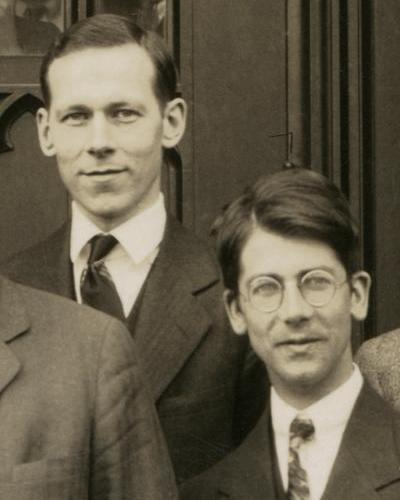
\includegraphics[width=\linewidth]{images/book3/mulliken-hund.jpg}
\end{minipage}\hfill
\begin{minipage}[t]{0.69\linewidth}
\vspace{0pt}
بين 1926 و1932 فسّر فريدريش هوند وروبرت موليكن أطياف
الجزيئات الثنائية الذرة بإسناد كل إلكترون إلى مدار يخص الجزيء
كله، مصنَّف وفق تناظره حول المحور. والكلمات $\sigma$ و$\pi$،
والرابط والمضاد للربط، ومخططات المدارات في هذا الفصل تأتي من
عملهما؛ ونال موليكن جائزة نوبل في الكيمياء سنة 1966. وتُظهر الصورة
موليكن (على اليسار) وهوند في شيكاغو سنة 1929. (صورة: غ. ف. هوند، CC~BY~3.0،
ويكيميديا كومنز.)
\end{minipage}
\end{history}

\section{التأين وقوة الرابطة}

نزع إلكترون من \omterm{def:b2:diatomic-mos:bonding}{مدار رابط} يُضعف الرابطة؛ ونزعه من
\omterm{def:b2:diatomic-mos:bonding}{مدار مضاد للربط} يقويها. وتأتي طاقات تفكك الأيونات
من دورة ترموكيميائية: فمن أجل $\mathrm{AB}^+ \to \mathrm A + \mathrm B^+$،
\[
  D_0(\mathrm{AB}^+) = D_0(\mathrm{AB}) + I(\mathrm B) - I(\mathrm{AB}) ,
\]
حيث B هي الذرة ذات طاقة التأين الأدنى.

\begin{example}[أيونا النيتروجين والأكسجين]\label{ex:b2:diatomic-mos:ions}
يفقد \ce{N2} ($I = \qty{15.58}{eV}$) إلكترونًا رابطًا: $D_0(\ce{N2+}) = 9.76 + 14.53 -
15.58 = \qty{8.71}{eV}$، أضعف من \ce{N2}. ويفقد \ce{O2} ($I = \qty{12.07}{eV}$)
إلكترون $\pi^*$: $D_0(\ce{O2+}) = 5.12 + 13.62 - 12.07 = \qty{6.66}{eV}$، أقوى من \ce{O2}،
بما يتفق مع رتبتي الرابطة 2.5 و2.5 مقابل 3 و2.
% ledger: ie:N2, ie:N, ie:O2, ie:O, janafH0:N, janafH0:O
\end{example}

\section{تمارين}

\begin{exercise}[$\star$]\label{exo:b2:diatomic-mos:1}
من أجل مداري 1s للهيدروجين خذ $\alpha = \qty{-13.6}{eV}$، و$\beta = \qty{-9.0}{eV}$ 
و$S = 0.60$ (معطيات تمرين). احسب $E_+$ و$E_-$، ثم طاقة إلكتروني
\ce{H2} مقارنة بذرتين منفصلتين.
\end{exercise}

\begin{exercise}[$\star$]\label{exo:b2:diatomic-mos:2}
أعطِ رتب الرابطة في \ce{He2} و\ce{He2+} و\ce{Li2} و\ce{B2} (مع مزج
s--p).
\end{exercise}

\begin{exercise}[$\star$]\label{exo:b2:diatomic-mos:3}
أي الجزيئات \ce{B2} و\ce{C2} و\ce{N2} و\ce{O2} و\ce{F2} \omterm{def:b2:diatomic-mos:magnetism}{بارامغناطيسية}؟
\end{exercise}

\begin{exercise}[$\star$]\label{exo:b2:diatomic-mos:4}
المحور الجزيئي هو $z$. أي الأزواج بين (1s، $2\mathrm p_z$)، و(1s،
$2\mathrm p_x$)، و($2\mathrm p_x$، $2\mathrm p_x$)، و($2\mathrm p_x$، $2\mathrm p_y$)،
و(2s، $2\mathrm p_z$) تداخلها غير معدوم؟
\end{exercise}

\begin{exercise}[$\star\star$]\label{exo:b2:diatomic-mos:5}
تنبأ هل رابطة \ce{N2+} أطول أم أقصر من رابطة \ce{N2}، وتحقق من ذلك بطاقة
تفككه المحسوبة في الفصل.
\end{exercise}

\begin{exercise}[$\star\star$]\label{exo:b2:diatomic-mos:6}
أحادي أكسيد الكربون و\ce{N2} متساويا الإلكترونات. فسّر لماذا تكون \omterm{def:b2:diatomic-mos:bonding}{المدارات الرابطة}
للجزيء CO مرجَّحة على الأكسجين ولماذا يكون أعلى مداراته المشغولة زوجًا حرًا على
الكربون.
\end{exercise}

\begin{exercise}[$\star\star$]\label{exo:b2:diatomic-mos:7}
في HF، أي مدارات الفلور تتآثر مع المدار 1s للهيدروجين، وأيها يبقى
غير رابط؟ ارسم المخطط.
\end{exercise}

\begin{exercise}[$\star\star$]\label{exo:b2:diatomic-mos:8}
مع $\alpha_A = \qty{-10}{eV}$، و$\alpha_B = \qty{-14}{eV}$ و$\beta = \qty{-3.0}{eV}$
(معطيات تمرين، مع إهمال $S$)، احسب الطاقتين ووزن $c_B^2$
\omterm{def:b2:diatomic-mos:bonding}{المدار الرابط} على B.
\end{exercise}

\begin{exercise}[$\star\star$]\label{exo:b2:diatomic-mos:9}
مع مزج s--p، بيّن أن \omterm{def:b2:diatomic-mos:bond-order}{رتبة الرابطة} في \ce{C2} تساوي 2 مكوّنة من رابطتي $\pi$ ودون
رابطة $\sigma_{2p}$.
\end{exercise}

\begin{exercise}[$\star\star\star$]\label{exo:b2:diatomic-mos:10}
أعطِ رتبتي الرابطة في NO و\ce{NO+}. وانطلاقًا من $D_0(\ce{NO}) = \qty{6.51}{eV}$، و$I(\ce{NO}) =
\qty{9.26}{eV}$ و$I(\ce{O}) = \qty{13.62}{eV}$، احسب $D_0(\ce{NO+})$ للتفكك $\ce{NO+} \to
\ce{N} + \ce{O+}$، وعلّق.
\end{exercise}

\begin{exercise}[$\star\star\star$]\label{exo:b2:diatomic-mos:11}
بيّن أن $E_+ + E_- = 2(\alpha - \beta S)/(1 - S^2)$، وأنه يتجاوز $2\alpha$ حين
$\beta < \alpha S < 0$. واستنتج لماذا يتنافر مداران ممتلئان (عدم الاستقرار
ذو الإلكترونات الأربعة).
\end{exercise}

\begin{exercise}[$\star\star\star$]\label{exo:b2:diatomic-mos:12}
رتّب \ce{O2+} و\ce{O2} و\ce{O2-} و\ce{O2^2-} وفق \omterm{def:b2:diatomic-mos:bond-order}{رتبة الرابطة} وطول الرابطة وقوة
الرابطة. أي أيون يوجد في بيروكسيد الهيدروجين، وأيها في المركب
الأصفر \ce{KO2}؟
\end{exercise}

\section{مسألة: الأكسجين وأيوناته}

\begin{problem}[{مسألة نهاية الأسبوع --- مخطط المدارات الجزيئية لثنائي الأكسجين،
ورتب الرابطة ومغناطيسية أيوناته، والتأين وقوة
الرابطة، والطريقتان لتوزيع إلكتروني $\pi^*$}]
\label{pb:b2:diatomic-mos:1}
المعطيات: $I(\ce{O}) = \qty{13.62}{eV}$، $I(\ce{O2}) = \qty{12.07}{eV}$، $I(\ce{N}) =
\qty{14.53}{eV}$، $I(\ce{N2}) = \qty{15.58}{eV}$؛ $\Delta_f H_0$ عند \qty{0}{K}
(\unit{kJ/mol}): \ce{O} 246.79، \ce{N} 470.82؛ $r_e$: \ce{O2} \qty{120.8}{pm}، \ce{N2}
\qty{109.8}{pm}؛ $1\ \unit{eV} = \qty{96.485}{kJ/mol}$.
% ledger: ie:O, ie:O2, ie:N, ie:N2, janafH0:O, janafH0:N, re:O2, re:N2

\medskip
\noindent\textbf{الجزء الأول --- ثنائي الأكسجين.}
\begin{enumerate}
  \item كم إلكترون تكافؤ في \ce{O2}؟
  \item ارسم مخطط \omterm{def:b2:diatomic-mos:lcao}{مداراته الجزيئية} التكافؤية (دون مزج s--p) واملأه.
  \item احسب \omterm{def:b2:diatomic-mos:bond-order}{رتبة الرابطة} فيه.
  \item كم إلكترونًا منفردًا؟ هل \ce{O2} \omterm{def:b2:diatomic-mos:magnetism}{بارامغناطيسي}؟
  \item لماذا تخفق بنية لويس هنا؟
  \item احسب $D_0(\ce{O2})$ بوحدة \unit{eV}.
\end{enumerate}

\medskip
\noindent\textbf{الجزء الثاني --- الأيونات.}
\begin{enumerate}[resume]
  \item أعطِ توزيع \ce{O2+} \omterm{def:b2:diatomic-mos:bond-order}{ورتبة الرابطة} فيه.
  \item والسؤال نفسه لأيون الأكسيد الفائق \ce{O2-}.
  \item والسؤال نفسه لأيون البيروكسيد \ce{O2^2-}.
  \item أعطِ عدد الإلكترونات المنفردة لكل أيون.
  \item رتّب \ce{O2+} و\ce{O2} و\ce{O2-} و\ce{O2^2-} وفق طول الرابطة المتنبأ به.
  \item أي أيون فيه رابطة O--O أحادية، كما في بيروكسيد الهيدروجين؟
  \item أي الأنواع الأربعة \omterm{def:b2:diatomic-mos:magnetism}{بارامغناطيسية}؟
\end{enumerate}

\medskip
\noindent\textbf{الجزء الثالث --- التأين.}
\begin{enumerate}[resume]
  \item من أي مدار يغادر الإلكترون حين يتأين \ce{O2}؟
  \item لماذا تكون $I(\ce{O2})$ أدنى من $I(\ce{O})$؟
  \item بيّن أن $D_0(\ce{O2+}) = D_0(\ce{O2}) + I(\ce{O}) - I(\ce{O2})$ واحسبها.
  \item قارن بالقيمة $D_0(\ce{O2})$ وفسّر.
  \item احسب $D_0(\ce{N2})$ و$D_0(\ce{N2+})$ بالطريقة نفسها.
  \item لماذا تكون $I(\ce{N2})$ أعلى من $I(\ce{N})$؟
  \item لخّص: متى يقوي التأين رابطة؟
\end{enumerate}

\medskip
\noindent\textbf{الجزء الرابع --- إلكترونا $\pi^*$.}
\begin{enumerate}[resume]
  \item في الحالة الأساسية يشغل إلكترونا $\pi^*$ مدارين مختلفين بسبينين
        متوازيين. أي قاعدة تقول ذلك؟
  \item صِف حالة يشغل فيها كلاهما مدار $\pi^*$ نفسه.
  \item لماذا تكون هذه الحالة أعلى طاقة؟
  \item ما \omterm{def:b2:diatomic-mos:bond-order}{رتبة الرابطة} فيها وما مغناطيسيتها؟
  \item اذكر \omterm{def:b2:diatomic-mos:bond-order}{رتبة الرابطة} في \ce{O2+} وطاقة تفككه.
\end{enumerate}
\end{problem}
